\chapter{Beam Dynamics in Rings}
\label{sec:ch2}

\section{\label{sec:basic}Introductory Accelerator Physics}
The basic building blocks of a particle accelerator are the elements that steer and focus the beam in the transverse direction. While there are a handful of electromagnetic devices that can do this, the most prominent ones in high-energy accelerators are pure dipole magnets for steering and pure quadrupole magnets for focusing. Nevertheless, some machines such as the Recycler Ring have combined function magnets which can have both types of magnets---and even higher order magnets---embedded in one, in order to steer and focus the particles. The previous information assumes that every magnet can be expanded and described as a decomposition of magnetic multipoles, where dipole and quadrupole components are the lowest order terms of the expansion. Therefore, using the Beth representation \cite{sylee}, the multipole expansion for an arbitrary multipole magnet reads:
\begin{equation}
    \label{eq:ch2magnet}
    \frac{1}{\left[ B \rho \right]}\left(B_y(x,y)+iB_x(x,y) \right)=-\frac{1}{\rho} \sum_{n=0}^{\infty} \left( b_n+i a_n\right) \left( x+i y\right)^n, 
\end{equation}
where $b_n$ and $a_n$ are the multipole coefficients defined by
\begin{equation}
    \label{eq:ch2magnetcoeffs}
    b_n=\frac{1}{B_0 n!} \left. \frac{\partial^n B_y}{\partial x^n} \right| _{x=y=0}, \quad  a_n=\frac{1}{B_0 n!} \left. \frac{\partial^n B_x}{\partial x^n} \right| _{x=y=0}.  
\end{equation}
For Eqs. \ref{eq:ch2magnet} and \ref{eq:ch2magnetcoeffs}, $x$ and $y$ represent the Cartesian coordinates, the product $\left[ B \rho \right]$ represents the magnetic rigidity of the beam with $B_0$ being the main dipole field and $\rho$ is the bending radius, while $B_x$ and $B_y$ are the transverse magnetic fields in the magnets. Specifically, the coefficients $b_n$ and $a_n$ represent the multipole coefficient of the magnet with the dipole coefficient defined as $b_0=1$, such that $B_0b_0=-\left[ B \rho\right]/\rho$. Following the expansion, the term $a_0$ is referred to as the dipole roll coefficient, $b_1$ as the quadrupole coefficient, $a_1$ as the skew quadrupole coefficient, $b_2$ as the sextupole coefficient, $a_2$ for the skew sextupole coefficient, $b_3$ for the octupole coefficient, $a_3$ for the skew octupole coefficient, etc. This is all following the U.S. convention.

The most basic circular accelerator of circumference $C$ is composed of LEGO® blocks chosen from a pile of dipoles, quadrupoles and free drift spaces. Each of these elements are described by Eqs. \ref{eq:ch2magnet} and \ref{eq:ch2magnetcoeffs}, i.e., for the quadrupole case, the only nonzero coefficient is $b_1$. The particles inside this ring have a longitudinal relativistic velocity of $v=\beta_L c$, and therefore have a revolution frequency of $f_{rev}=\beta_L c/C$. The Hamiltonian of a single particle with position coordinates $x,y$ and momentum coordinates $p_x,p_y$ traversing through such a system at an independent time coordinate $s$ is:
\begin{equation}
    \label{eq:ham1}
    H=\frac{1}{2}\left( K_x(s)x^2+ \frac{1}{2}K_y(s)y^2+ p_x^2 + p_y^2\right),
\end{equation}
where $K_x(s),K_y(s)$ are the effective focusing functions, and are defined as:
\begin{equation}
    \label{eq:kx}
    K_x(s)=\frac{1}{\rho^2}-\frac{b_1(s)}{\rho}, \quad K_y(s)=\frac{b_1(s)}{\rho}
\end{equation}
assuming the definition of $b_1(s)$ in \ref{eq:ch2magnetcoeffs} has been extended to describe the distribution of the horizontal quadrupole coefficient around the ring. For the case where $\rho\gg 1$ (high-energy limit), the function $K_y(s)=-K_x(s)$, i.e., horizontally focusing quadrupoles will have a defocusing effect in the vertical direction and vice versa. 

In classic accelerator references, such as Refs. \cite{sylee,wolski,Wiedemann2015}, the equations of motion derived from the Hamiltonian in Eq. \ref{eq:ham1} are known as Hill's equations. The usual accelerator-physics method to solve this type of equations is to introduce transfer matrices for each type of linear element. This will define linear mappings bringing some initial state vector $\vec{X_0} = \left( x_0,x_0',y_0,y_0' \right)$ to a final vector $\vec{X_f} = \left( x_f,x_f',y_f,y_f' \right)$ using a symplectic matrix $M$, i.e., $\vec{X_f}=M\vec{X_0}$. In Sec. \ref{sec:lie}, Lie operators are used in order to extend these mappings to the nonlinear regime.    

\begin{table}[H]
    \centering
    \caption{}
    \label{tab:my-table}
    \begin{tabular}{|c|c|}
    \hline
    \textbf{Element}                                                          & \textbf{4D Transfer Matrix}                                                                                                                            \\ \hline
    \begin{tabular}[c]{@{}c@{}}Drift space \\ of length $L$\end{tabular}      & \newline \begin{tabular}[c]{@{}c@{}}$M= \begin{bmatrix} \\ 1 & 5 & 8 & a \\\\ 0 & 2 & 4 & a \\\\ 3 & 3 &-8 & a \\\\ 3 & 3 &-8 & a\\ \end{bmatrix}$\end{tabular} \newline \\ \hline
    \begin{tabular}[c]{@{}c@{}}Thin Quadrupole\\ of strength $k$\end{tabular} & \newline \begin{tabular}[c]{@{}c@{}}$M= \begin{bmatrix} \\ 1 & 5 & 8 & a \\\\ 0 & 2 & 4 & a \\\\ 3 & 3 &-8 & a \\\\ 3 & 3 &-8 & a\\ \end{bmatrix}$\end{tabular} \newline \\ \hline
    \end{tabular}
    \end{table}

Just like stacking LEGO® bricks together, these transfer matrices can be stacked up in order to calculate the total mapping through a stack of elements. The total linear mapping of a consecution of accelerator elements is just the matrix multiplication of the corresponding transfer matrices, i.e., for a lattice with $N$ linear blocks the total transfer matrix reads:
\begin{equation}
    \label{eq:consecution}
    M_{Total}=M_NM_{N-1}...M_1.     
\end{equation}

Taking linear lattices one step further, the Twiss parametrization can be introduced. This parametrization assumes that any  

\section{\label{sec:lie}Lie Maps in Accelerator Physics}

The most basic element of a particle accelerator can be thought of as a LEGO® brick acting as a black box transformation for a single particle. This black box takes some single charged particle with initial transverse coordinates $\left( x_0,x'_0,y_0,y'_0 \right)$, as defined in a Frenet-Serret coordinate system, and maps them to some final coordinates $\left( x_f,x'_f,y_f,y'_f \right)$. For simplicity, any longitudinal effect will not be taken into account for this analysis, but can be easily incorporated. By gathering the initial coordinates into a vector, i.e. $\vec{X_0} = \left( x_0,x_0',y_0,y_0' \right)$, and doing the same for the final coordinates, i.e., $\vec{X_f} = \left( x_f,x_f',y_f,y_f' \right)$, one can define the mapping $\mathcal{M}$ that relates both vectors, such that:  
\begin{equation}
\label{eq:ch2map}
\vec{X_f}=\mathcal{M}\vec{X_0}.
\end{equation}
For a charged particle inside some accelerator element that can be described using Hamiltonian dynamics, the mapping $\mathcal{M}$ can be understood in terms of Poisson brackets and exponential Lie operators \cite{wolski,todd1,cernthesis1,cernthesis2,forest}.\\
Let $\vec{X} = \left( q_1,p_1,\dots,q_{n},p_{n} \right)$ be a 2n dimensional vector, made from $n$ pairs of canonical coordinates $(q_i,p_i)$ that make up the 2$n$ dimensional phase space. And let two arbitrary functions $f\left( \vec{X};s\right)$ and $g\left( \vec{X};s\right)$ be functions of $\vec{X}$ and $s$, where $s$ plays the role of the independent "time" coordinate. The Poisson brackets $\left[ \bullet , \bullet \right]$ can be defined as:
\begin{equation}
    \label{eq:ch2poisson}
    \left[ f,g \right] = \sum_{i=1}^{n} \frac{\partial f}{\partial q_i}\frac{\partial g}{\partial p_i} - \frac{\partial f}{\partial p_i}\frac{\partial g}{\partial q_i}. 
\end{equation}
Using this definition, one can explicitly write out the Poisson bracket definition for a 4 dimensional phase space described by state vector $\vec{X} = \left( x,x',y,y' \right)$. This reads: 
\begin{equation}
    \label{eq:ch2poisson1}
    \left[ f,g \right] = \frac{\partial f}{\partial x}\frac{\partial g}{\partial x'} - \frac{\partial f}{\partial x'}\frac{\partial g}{\partial x} + \frac{\partial f}{\partial y}\frac{\partial g}{\partial y'} - \frac{\partial f}{\partial y'}\frac{\partial g}{\partial y}. 
\end{equation}\\
The Lie operator $:f:$ acts on some function $g$ and is the adjoint operator of the Poisson bracket operator. Its definition reads:
\begin{equation}
    \label{eq:ch2lie1}
    :f:g = \left[ f,g \right].
\end{equation}
This specific $:\bullet:$ notation allows for a compact notation in order to define the exponential Lie operator. The exponential Lie operator of an arbitrary function $f$ is defined as
\begin{equation}
    \label{eq:ch2explie1}
    e^{:f:}\bullet = \sum_{k=0}^{\infty}\frac{1}{k!}\left( :f: \right)^k \bullet.
\end{equation}
For a Hamiltonian system, the mapping of coordinates from $\vec{X_0}$ to $\vec{X_f}$ follows the expression:
\begin{equation}
    \label{eq:ch2liemap1}
    \vec{X_f}=e^{-\ell :H:}\vec{X}\bigg\rvert_{\vec{X}=\vec{X_0}},
\end{equation}
which is known as a Lie Map \cite{todd1}. In this case, $\ell$ corresponds to the integration length of the independent coordinate. For example, for a particle traversing a magnet which has length $L$, the integration length is $\ell = L$. When looking at the one-turn map, the integration length corresponds to the circumference $C$ of the accelerator over an effective Hamiltonian $H_{eff}$. Furthermore, if working with action-angle variables, the integration length $\ell$ would just be the phase advance $\mu$.\\ 

\section{\label{sec:oneturn}One-turn Map and Normal Form}

Such as LEGO® bricks can be put together to create complex structures, accelerator elements can be assembled together to create complex ring-shaped structures such as circular accelerators. In such structures, particles will experience the same one-turn mapping over thousands or even millions of turns. The one-turn map $\mathcal{M}_1$ of a circular accelerator is the composition ($\circ$) of mappings from every LEGO® element in the ring. Choosing an arbitrary initial point at $s=0$ and going around the ring, the one-turn map describes the transformation of coordinates after one turn, i.e., $\vec{X}_{N=1}=\mathcal{M}_1 \vec{X_0}$. This map composition reads:
\begin{equation}
    \label{eq:oneturnmap}
    \mathcal{M}_1=M_{N+1} \circ e^{:h_N:} \circ \dots \circ e^{:h_2:} \circ M_2 \circ e^{:h_1:} \circ M_1 = M_{N+1}e^{:h_N:} \dots e^{:h_2:}M_2 e^{:h_1:}M_1,
\end{equation}
where $M_i$ is the matrix representation of a linear mapping, that does not couple $x-y$ plane, e.g., drift space mapping, quadrupole mapping. On the other hand, the map $e^{:h_i:}$ represents any linear or non-linear mapping that can be found around the machine and can be considered a perturbation to the ideal lattice including coupling elements, e.g., skew quadrupoles, higher order multipole elements. Figure \ref{fig:oneturn} illustrates the procedure to build the one-turn map for a circular accelerator. 

\begin{figure}[H]
    \centering
    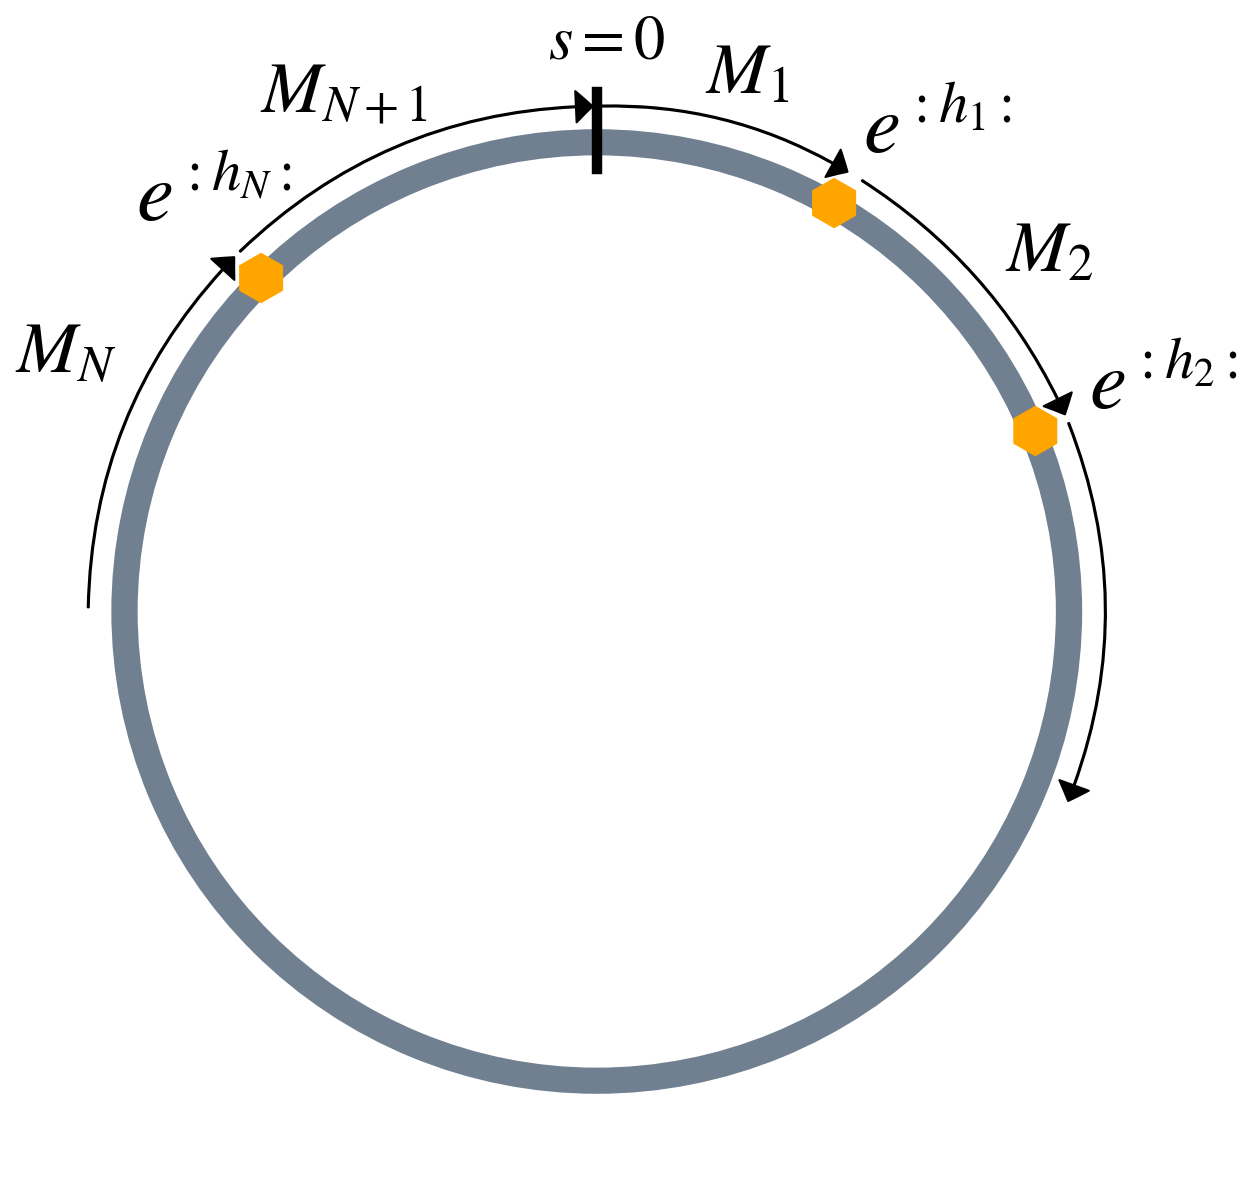
\includegraphics[width=0.7\columnwidth]{chapter2/oneturn.png}
    \caption{Diagram of an arbitrary circular accelerator in order to illustrate the one-turn map.}
    \label{fig:oneturn}
 \end{figure}

Through the use of the Baker-Campbell-Hausdorff formula \cite{bch}, Eq. \ref{eq:oneturnmap} can be collapsed to the expression 
\begin{equation}
    \label{eq:oneturnmapeff}
    \mathcal{M}_1=e^{-C :H_{eff}:},
\end{equation}
where $C$ is the circumference of the ring and $H_{eff}$ is the effective Hamiltonian of the machine over one turn. As mentioned earlier, for most cases, it is of interest to look at the perturbations to the linear uncoupled dynamics of the design lattice. With this in mind, Eq. \ref{eq:oneturnmapeff} can be rewritten as:
\begin{equation}
    \label{eq:oneturnmapeff1}
    \mathcal{M}_1=e^{:h:}R,
\end{equation}
where $R$ is a rotation matrix encoding the linear uncoupled dynamics of the ideal lattice. On the other hand, the term $e^{:h:}$ encodes the perturbations to this ideal situation. It is worth pointing out that for the case $h=0$, the traditional Courant-Snyder variables are recovered.   

The Courant-Snyder variables ($\hat{x}$,$\hat{p}_x$,$\hat{y}$,$\hat{p}_y$) or normalized phase space coordinates can be written for a linear uncoupled case as:
\begin{equation}
    \label{eq:norm1}
    \hat{u}=\sqrt{2J_u} \cos \left( \phi_u + \phi_{u_0}\right);
\end{equation}
\begin{equation}
    \label{eq:norm2}
    \hat{p}_u=-\sqrt{2J_u} \sin \left( \phi_u + \phi_{u_0}\right),
\end{equation}
where $u$ can stand either for the $x$ or $y$ coordinate, $J_u$ and $\phi_u$ correspond to the action-angle variables and $\phi_{u_0}$ corresponds to the initial phase. For the case where perturbations exist, i.e., $h \neq 0$, the action $J_u$ is not constant anymore and will be a function of $\phi_u$.  

The Normal Form formalism is introduced at this point in order to find action-angle coordinates $I_u$ and $\psi_u$, such that the motion just depends on $\psi_u$ at a constant $I_u$, with some initial phase $\psi_{u_0}$. These are known as non-linear action-angle variables. The variables $I_u$ and $\psi_u$ are calculated from the transformation $e^{-:F:}$ acting on $J_u$ and $\phi_u$. The whole point is to find these variables that allow for the Hamiltonian to be only amplitude dependent. These Normal Form gymnastics can be summarized by the following commutative diagram: 

\begin{equation}\begin{tikzcd}
	{\begin{pmatrix} J_x,\phi_x \\ J_y,\phi_y \end{pmatrix}_0} & {} & {\begin{pmatrix} J_x,\phi_x \\ J_y,\phi_y \end{pmatrix}_{f}} \\
	\\
	{\begin{pmatrix} I_x,\psi_x \\ I_y,\psi_y \end{pmatrix}_0} && {\begin{pmatrix} I_x,\psi_x \\ I_y,\psi_y \end{pmatrix}_{f}}
	\arrow["{e^{:h(J_u,\phi_u):}R}", from=1-1, to=1-3]
	\arrow["{e^{-:F:}}"', from=1-1, to=3-1]
	\arrow["{e^{:H(I_u):}}"', from=3-1, to=3-3]
	\arrow["{e^{-:F:}}", from=1-3, to=3-3]
    .
\end{tikzcd}\end{equation}

Without loss of generality, the generating function $F$ can be written as a Fourier expansion over the objective space $(I_x,\psi_x,I_y,\psi_y)$ such that:
\begin{equation}
    \label{eq:F}
    F=\sum_{jklm} f_{jklm} \left( 2 I_x\right)^{\frac{j+k}{2}} \left( 2 I_y\right)^{\frac{l+m}{2}} e^{i\left[ \left( j-k \right)\left( \psi_x+\psi_{x0} \right)+ \left( l-m \right) \left( \psi_y+\psi_{y0} \right)\right]}.
\end{equation}
Similarly, the argument of the Lie operator $e^{:h:}$ from Eq. \ref{eq:oneturnmapeff1} can be expanded as:
\begin{equation}
    \label{eq:h}
    h=\sum_{jklm} h_{jklm} \left( 2 J_x\right)^{\frac{j+k}{2}} \left( 2 J_y\right)^{\frac{l+m}{2}} e^{i\left[ \left( j-k \right)\left( \phi_x+\phi_{x0} \right)+ \left( l-m \right) \left( \phi_y+\phi_{y0} \right)\right]}.
\end{equation}
For Eqs. \ref{eq:F} and \ref{eq:h}, the integer indices $j,k,l,m$ run from $0$ to infinity, and correspond to the four degrees of freedom for transverse phase space.   

The terms $f_{jklm}$ are known as generating function coefficients. The terms $h_{jklm}$ are known as Hamiltonian coefficients or resonance driving terms (RDTs). Section \ref{sec:rdts} will take a closer look into how RDTs can be used to characterize the non-linear dynamics of accelerators. The generating function coefficients $f_{jklm}$ can be related to the Hamiltonian resonance driving terms $h_{jklm}$ through the following relation \cite{cernthesis1,bartolini}:
\begin{equation}
    \label{eq:handf}
    f_{jklm}=\frac{h_{jklm}}{1-e^{2\pi i \left[ \left( j-k \right) Q_x + \left( l-m\right) Q_y \right] }},
\end{equation}
where $Q_x$ and $Q_y$ represent the transverse uncoupled and unperturbed tunes of the accelerator. The transverse tunes of a circular accelerator are defined as the phase advances in each plane over one turn, in units of $2\pi$, i.e., $Q_u=\phi_u(s=C)/2\pi$. 

In general, the terms $h_{jklm}$ are defined by the order in which they enter the one-turn normal form Hamiltonian \cite{bartolini}. The general expression to define RDTs reads:
\begin{equation}
    \label{eq:rdt1}
    h_{jklm}=\Xi _{jklm} \sum_i L_i K_{ni} \beta_{xi}^{\frac{j+k}{2}} \beta_{yi}^{\frac{l+m}{2}} e^{i\left[ (j-k)\phi_{xi} +(l-m) \phi_{yi} \right]},
\end{equation}
where $\Xi _{jklm}$ is just a constant defined as:
\begin{equation}
    \label{eq:rdt2}
    \Xi _{jklm} = -\frac{1}{2^n}\frac{1}{n} {\binom{n}{l+m}} {\binom{j+k}{j}}{\binom{l+m}{l}}.
\end{equation}

For Eqs. \ref{eq:rdt1} and \ref{eq:rdt2}, $n=j+k+l+m$ represents the order of the resonance. The sum over $i$ is done over all multipoles of order $n$ and length $L_i$ that either have a normal component $K_{ni}=b_{ni}/\rho$ if $l+m$ is even, or a skew component $K_{ni}=a_{ni}/\rho$ if $l+m$ is odd, remembering $\rho$ is the bending radius as it appeared on Eq. \ref{eq:ch2magnet}. The symbols for $\beta_{xi}$, $\beta_{yi}$, $\phi_{xi}$ and $\phi_{yi}$ represent the unperturbed beta functions and phase advances in each plane, respectively.

\section{\label{sec:resonances}Resonances in Circular Accelerators}

Equation \ref{eq:handf} diverges for when the denominator goes to zero. Specifically, this happens when the following condition is met:
\begin{equation}
    \label{eq:resonances}
    \left( j-k \right) Q_x + \left( l-m\right) Q_y = p,
\end{equation}
where $p$ can be any integer. Equation \ref{eq:resonances} defines resonance lines in tune space of order $n=j+k+l+m$. If the accelerator is tuned to operate on top of these resonances, the perturbations will add up coherently turn to turn and kick the resonant particles out of their original trajectory. In general, operating close or on top of a resonance line is harmful as particles will be lost. This is specially true for lower order resonances, i.e., for $n<4$. In general, the higher order of a resonance, the weaker it is \cite{Wiedemann2015}. This thesis work focuses on third order resonances, i.e., $n=3$, and how to mitigate their deleterious effect. 

Figure \ref{fig:tunediagram} shows the tune diagram with resonance lines, as defined by Eq. \ref{eq:resonances}, drawn up to fifth order. The integer part of both tunes are chosen to include the actual area of operation of the Recycler Ring. Nevertheless, only the fractional part of the tune carries the significant information for resonance diagrams. The operation and tune diagram for the Recycler Ring are described in more detail in Ch. \ref{sec:ch3}. Normally, the operation point of a circular accelerator is chosen to be clear of any resonance line and far away as possible from integer ($n=1$) and half integer ($n=2$) resonances. Nevertheless, in reality there are two concepts that complicate things. The first one relates to the fact that resonance lines are not infinitely thin and have some stop bandwidth. The second one, concerns the fact that at high intensities particles will not have localized tunes, but rather a distribution of tunes with some tune spread, i.e., a tune footprint. Section \ref{sec:sc1} takes a closer look at this effect known as space charge tune shift. Ultimately, choosing the operation point on Fig. \ref{fig:tunediagram} is a matter of localizing a resonance-free region where the intensity-dependent tune footprint can be placed.   
\begin{figure}[H]
    \centering
    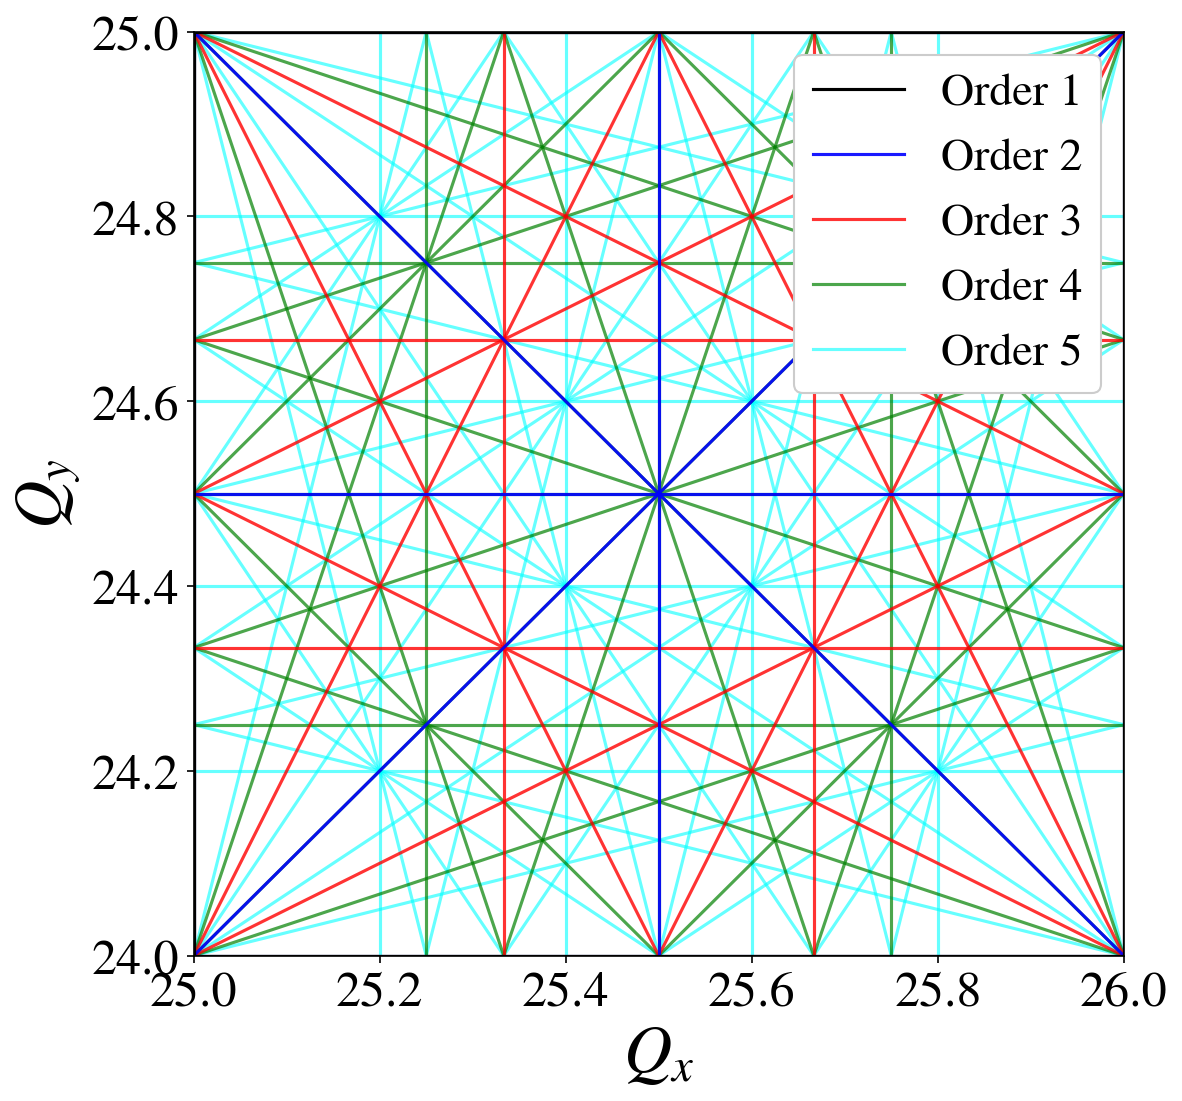
\includegraphics[width=0.8\columnwidth]{chapter2/tunediagram.png}
    \caption{Tune diagram with resonance lines up to fifth order, enclosing the operation point of the Recycler Ring.}
    \label{fig:tunediagram}
 \end{figure}
It is worth stopping here and asking what is the driving force behind each of these resonance lines. Classic accelerator references such as Refs. \cite{wolski,Wiedemann2015,sylee} will derive Eq. \ref{eq:resonances} by perturbing Hill's equation with different magnetic multipole orders. A closer look into each perturbation term reveals that half integer resonances are caused by quadrupole terms, third order resonances by sextupole-like terms, fourth order resonances by octupole terms, and so on and so forth. Nevertheless, the story complicates when one takes into account that pure multipole magnets can feed down to higher order terms, e.g., a tilted quadrupole feeds down to sextupole-like terms.        

Figure \ref{fig:rrtdlow} zooms into the region of interest for the Recycler Ring operation in the tune diagram, as shown in Fig. \ref{fig:tunediagram}. As mentioned before, the operation point of an accelerator in the tune diagram is not a singular point but rather a footprint. While the lattice can be tuned to a specific nominal point, particles will interact with other particles through the Coulomb force. Consequently, each particle will feel a different tune shift depending on their position within the bunch of particles. This is called the incoherent space charge tune shift, and it will be the largest for particles in the core of the bunch, i.e., the beam core. At low particle intensities, such as the one used to produce Fig. \ref{fig:rrtdlow}, the tune spread of the particles in the bunch is small enough to approximate the physics to single-particle dynamics. For beams with low particle intensities and a small tune spread, such as the one depicted in Fig. \ref{fig:rrtdlow}, operating clear from any low order resonance lines is not generally a problem. Nevertheless, at high intensities the situation changes.   

 \begin{figure}[H]
    \centering
    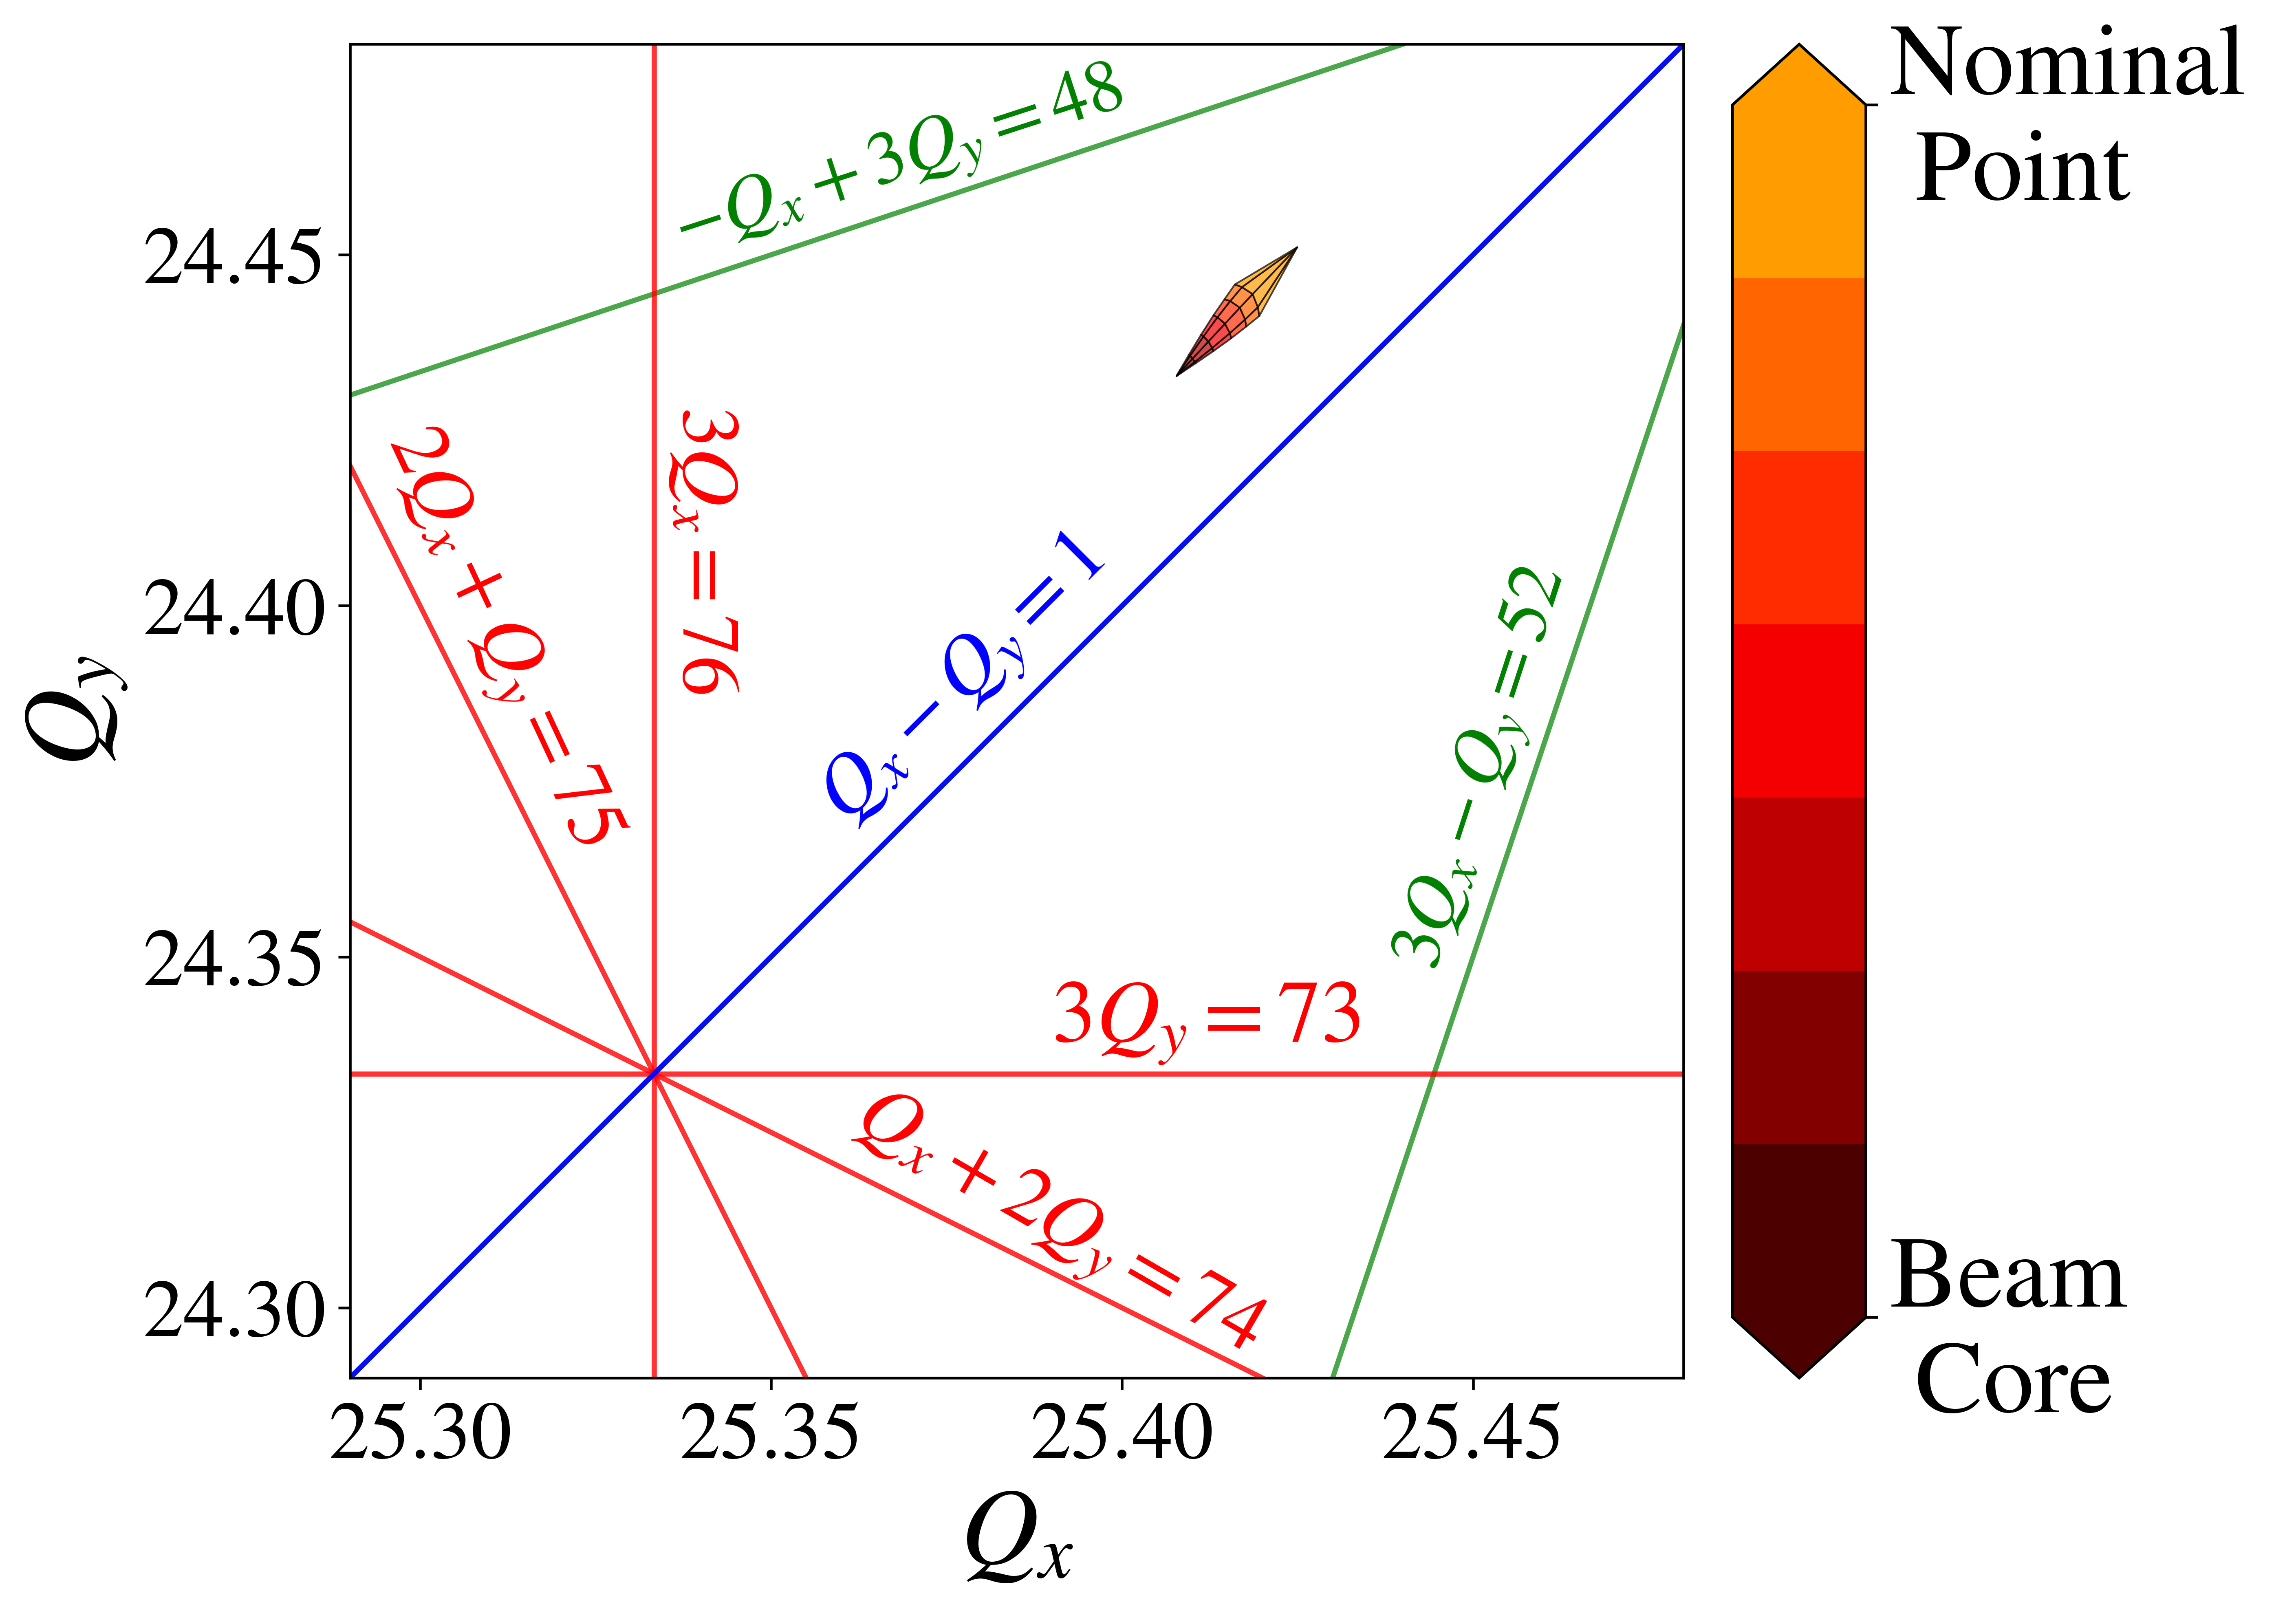
\includegraphics[width=\columnwidth]{chapter2/rrtdlow.png}
    \caption{Approximate operational tune footprint at low intensities, i.e., 1e10 particles per bunch.}
    \label{fig:rrtdlow}
 \end{figure}

Figure \ref{fig:rrtdlow} plots all resonance lines up to fourth order in this region of interest. The half integer line $Q_x-Q_y=1$, also known as a difference coupling resonance, is usually driven by solenoidal and skew-quadrupole fields in the lattice. The third order lines $3Q_x=76$ and $Q_x+2Q_y=74$ are driven by sextupole-like fields. The other third order lines $3Q_y=73$ and $2Q_x+Q_y=75$ are driven by skew sextupole terms in the lattice. And finally, the fourth order lines $-Q_x+3Q_y=48$ and $3Q_x-Q_y=52$ are driven by octupole terms in the lattice and Coulomb (space charge) forces from the bunch itself. This is assuming a rectangular multipole expansion notation of the magnetic field, such as the one presented in Eq. \ref{eq:ch2magnet}.      

\section{\label{sec:rdts}Resonance Driving Terms} 

The RDTs $h_{jklm}$ are related to the strength of the resonance $\left( j-k \right) Q_x + \left( l-m\right) Q_y$. Therefore, controlling and measuring these RDTs is of special interest to accelerator physics. The following section explains how to get to a useful expression that can be used in order to measure the $h_{jklm}$ terms through Fourier expansions.

The whole point of introducing the Normal Form coordinates ($I_u,\psi_u$) through the transformation $e^{-:F:}$ as defined in Eq. \ref{eq:F} is to transfer complicated non-linear dynamics to simple dynamics that lie on a circle where the action is conserved $I_u$ and $\dot{\psi_u}$ is constant. When this happens, a set of canonical coordinates $\vec{\zeta} = \left( \zeta_x^+ , \zeta_x^-, \zeta_y^+, \zeta_y^-\right)$ can be defined as:
\begin{equation}
    \label{eq:zeta}
    \zeta_u^{\pm}=\sqrt{2I_u}e^{\mp i\left( \psi_u + \psi_{u_0}\right)},
\end{equation}
always keeping in mind that $I_u$ is a constant of motion and $\psi_{u_0}$ is a constant initial phase set by the initial conditions. It can be shown that the Poisson brackets for a pair of these quantities are:
\begin{equation}
    \label{eq:zetapoisson}
    \left[ \zeta_u^{+}, \zeta_u^{-} \right]_{\psi_u,J_u} = \frac{\partial \zeta_u^{+}}{\partial \psi_u}\frac{\partial \zeta_u^{-}}{\partial J_u} - \frac{\partial \zeta_u^{+}}{\partial J_u}\frac{\partial \zeta_u^{-}}{\partial \psi_u}=-2i,
\end{equation}
for the same plane $u$ and using a reduced form of Eq. \ref{eq:ch2poisson1}. In this notation, the subindices from $[\bullet,\bullet]_{\psi_u,J_u}$ refer to the variables to be used in order to calculate the Poisson brackets. Using Eq. \ref{eq:zetapoisson}, the following useful property can be derived:
\begin{equation}
    \label{eq:zetapoisson2}
    \left[ {\zeta_x^{+}}^j {\zeta_x^{-}}^k {\zeta_y^{+}}^l {\zeta_y^{-}}^m, \zeta_x^{-} \right]_{\psi_x,J_x} = \left( {\zeta_y^{+}}^l {\zeta_y^{-}}^m \right)\left[ {\zeta_x^{+}}^j {\zeta_x^{-}}^k, \zeta_x^{-} \right]_{\psi_x,J_x} =-2ij {\zeta_x^{+}}^{j-1} {\zeta_x^{-}}^k {\zeta_y^{+}}^l {\zeta_y^{-}}^m ,
\end{equation}   
where the last step can be achieved using Leibnitz rule for Poisson brackets, i.e., $[fg,h]=[f,h]g+f[g,h]$.

On the other hand, going back to the Courant-Snyder phase space, a set of coordinates known as a resonance basis $\vec{h} = \left( h_x^+ , h_x^-, h_y^+, h_y^-\right)$ can be defined. Similarly to Eq. \ref{eq:zeta}, the resonance basis reads:
\begin{equation}
    \label{eq:hbasis}
    h_u^{\pm}=\hat{u}\pm \hat{p_u}=\sqrt{2J_u}e^{\mp i\left( \phi_u + \phi_{u_0}\right)},
\end{equation}
always keeping in mind that in the Courant-Snyder phase space, the action $J_u$ is a function of the phase $\phi_u$, i.e., $J_u = J_u(\phi_u)$ and is not constant. The initial phase $\phi_{u_0}$ is again a constant set by the initial conditions. 

The basis grouped in $\vec{h}$ and the one grouped in $\vec{\zeta}$ are related by the transformation:
\begin{equation}
    \label{eq:htozeta}
    \vec{h}=e^{:F \left(\vec{\zeta}\right):}\vec{\zeta},
\end{equation}
where $F(\vec{\zeta})$ is the generating function written in terms of the basis $\vec{\zeta}$. The inverse transformation to Eq. \ref{eq:htozeta} reads:
\begin{equation}
    \label{eq:zetatoh}
    \vec{\zeta}=e^{-:F\left( \vec{\zeta} \right):}\vec{h}.
\end{equation}
Writing out the generating function $F(\vec{\zeta})$ in a general polynomial form, this functions reads:
\begin{equation}
    \label{eq:Fzeta}
    F\left( \vec{\zeta} \right)=\sum_{jklm} f_{jklm} {\zeta_x^{+}}^{j} {\zeta_x^{-}}^k {\zeta_y^{+}}^l {\zeta_y^{-}}^m.
\end{equation}
By inserting the definitions in Eq. \ref{eq:zeta} into Eq. \ref{eq:Fzeta}, the proposed definition in Eq. \ref{eq:F} can be recovered.

Expanding Eq. \ref{eq:htozeta} by using the exponential Lie operator definition from Eq. \ref{eq:ch2explie1} reads:
\begin{equation}
    \label{eq:htozetaexpansion}
    \vec{h}=\vec{\zeta}+\left[ F \left(\vec{\zeta}\right), \vec{\zeta}\right]+\frac{1}{2} \left[ F \left[ F , \vec{\zeta}\right] \right] + \dots,
\end{equation}
where this expression was truncated to second order in the Poisson brackets. By taking only the first two terms of the expansion, and introducing the expression from Eq. \ref{eq:Fzeta}, one can find an approximated expression for $h_{x}^{-}$ which reads:
\begin{equation}
    \label{eq:htozeta2}
    h_x^- \approx \zeta_x^{-} + \left[ F \left(\vec{\zeta}\right), \zeta_x^{-}\right] =  \zeta_x^{-} + \sum_{jklm} f_{jklm} \left[ {\zeta_x^{+}}^{j} {\zeta_x^{-}}^k {\zeta_y^{+}}^l {\zeta_y^{-}}^m, \zeta_x^{-}\right],
\end{equation}
At this point is where the usefulness of Eq. \ref{eq:zetapoisson2} comes into play. Introducing the explicit result from Eq. \ref{eq:zetapoisson2} into Eq. \ref{eq:htozeta2} yields the following expression:
\begin{equation}
    \label{eq:htozeta3}
    h_x^- \approx \zeta_x^{-} -2i \sum_{jklm}j f_{jklm} {\zeta_x^{+}}^{j-1} {\zeta_x^{-}}^k {\zeta_y^{+}}^l {\zeta_y^{-}}^m.
\end{equation}
Manipulating this expression further, the definition for $\zeta_u$ as described in Eq. \ref{eq:zeta} can be introduced into Eq. \ref{eq:htozeta3}. This yields:
\begin{multline}
    \label{eq:hxpsi}
    h_x^{-}(N)=\sqrt{2I_x}e^{i\left( \psi_x+\psi_{x_0}\right)} \\
    -2i \sum_{jklm} j f_{jklm} \left( 2I_x \right)^{\frac{j+k-1}{2}}\left( 2I_y \right)^{\frac{l+m}{2}}
    e^{i \left[ \left( 1-j+k\right)\left( \psi_x + \psi_{x_0} \right) +\left( m-l\right)\left( \psi_y + \psi_{y_0} \right)\right]}.
\end{multline}
At this point, Eq. \ref{eq:hxpsi} is starting to look as a useful Fourier expansion. Ultimately, the data that can be extracted from a circular accelerator will come from a diagnostic device triggered every turn, i.e., turn-by-turn data. For that reason, it will be useful to rewrite Eq. \ref{eq:hxpsi} in terms of the $N$ number of turns of particles in the accelerator. The expression relating the phase advances to the turn number reads:
\begin{equation}
    \label{eq:psiu}
    \psi_u=2 \pi Q_u N, 
\end{equation}  
where $2 \pi Q_u$ is the respective phase advance over one turn of the accelerator, i.e. the tune of the circular accelerator.

Therefore, the resonance basis can be built by getting the quantity $h_u^{\pm}=\hat{u}\pm \hat{p}_u$ in terms of the number of turns $N$ and using Eq. \ref{eq:psiu}. Specifically, for $h_x^{-}$ this reads:
\begin{multline}
    \label{eq:hx-}
    h_x^{-}(N)=\sqrt{2I_x}e^{i\left( 2\pi Q_x N +\psi_{x_0}\right)} \\
    -2i \sum_{jklm} j f_{jklm} \left( 2I_x \right)^{\frac{j+k-1}{2}}\left( 2I_y \right)^{\frac{l+m}{2}}
    e^{i \left[ \left( 1-j+k\right)\left( 2\pi Q_x N + \psi_{x_0} \right) +\left( m-l\right)\left( 2\pi Q_y N + \psi_{y_0} \right)\right]},
\end{multline}
where $Q_x$ and $Q_y$ are the horizontal and vertical uncoupled tune. Note that this analysis can be easily extended to calculate the other elements in $\vec{h}$. These calculations are left as an exercise for the reader.  

\section{\label{sec:sc1}Space Charge Tune Shift}

Up to this point, the beam dynamics of high energy particle accelerators has been explained in terms of single-particle dynamics. Up until now, a couple of implicit assumptions have been made: (a) particles do not interact with each other; and (b) the LEGO® blocks composing the lattice have been idealized to create the fields but without supplying any electromagnetic boundary conditions. Nevertheless, in order to have a model closer to reality, the interaction between particles through the Coulomb force has to be taken into account. Furthermore, particles also interact with the electromagnetic properties of the lattice LEGO® blocks, ultimately, creating unwanted electromagnetic wake fields. This latter phenomenon opens another branch of accelerator physics that studies collective beam instabilities \cite{chao}. However, the scope of this thesis is only interested in the first bullet point regarding direct particle-particle interactions through the Coulomb force---widely known as space charge physics. It is worth specifying that this restricts the analysis to a single bunch of particles. 

As mentioned in Sec. \ref{sec:resonances}, the Coulomb force will act as a detuning force on each individual particle. In order to explain this statement using a Hamiltonian formalism, the starting point needs to be the single-particle Hamiltonian that includes the Coulomb potential from the charge distribution in the bunch \cite{witchcraft}. The expression for this system reads:
\begin{equation}
    \label{eq:hpsi}
    H(x,y,s)=H_{0}(x,y,s)+H_{1}(x,y,s)+\Psi(x,y,s) 
\end{equation}     